\documentclass[12pt]{beamer}
\mode<presentation>
\usepackage{algorithm}
\usepackage{algpseudocode}


\useinnertheme{rectangles}
\setbeamercolor*{item}{fg=red}
\setbeamercovered{transparent}
\usecolortheme{beaver}



\title{Finding Approximate Solutions to the Minimum Metric $p$-Center Problem on Graphs Using Ant Colony Optimization}
\author{James Carlo Plaras and Jaime Samaniego}
\date{}

\begin{document}
\maketitle

\begin{frame}
\frametitle{Outline}
\tableofcontents
\end{frame}

\AtBeginSection[]
{
\begin{frame}<beamer>{Outline}
\tableofcontents[currentsection,currentsubsection, 
    hideothersubsections, 
    sectionstyle=show/shaded,
]
\end{frame}
}
\AtBeginSubsection[]
{
\begin{frame}<beamer>{Outline}
\tableofcontents[currentsection,currentsubsection, 
    hideothersubsections, 
    subsectionstyle=show/shaded,
]
\end{frame}
}

\section{Introduction}
\begin{frame}
\frametitle{Motivation}
\begin{center}
Efficient \alert{facility location} is a well-known problem in computer science and operations research.
\end{center}
\end{frame}

\begin{frame}
\frametitle{Motivation}
\begin{center}
Very related to computational geometry and graph theory.
\end{center}
\end{frame}

\begin{frame}
\frametitle{Motivation}
\begin{center}
\textit{What is the \alert{best} placement of facilities in given candidate locations to minimize cost (or maximize profit)?}
\end{center}
\end{frame}

\begin{frame}
\frametitle{Facility Location}
\begin{center}
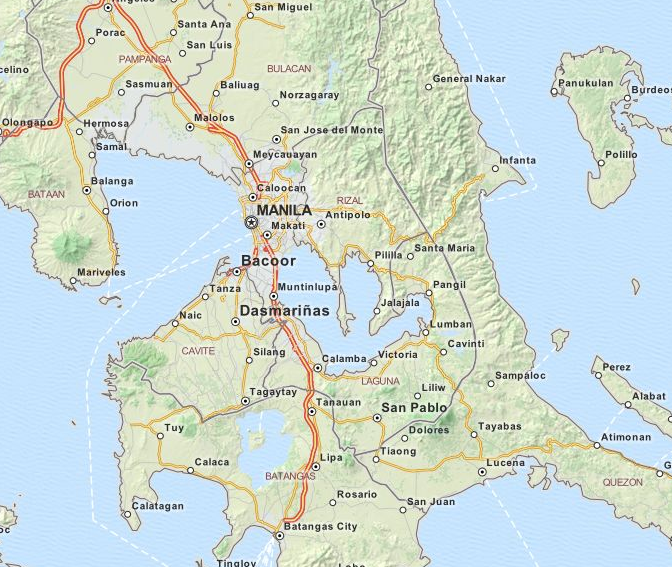
\includegraphics[height=75mm]{Images/Intro1}\\
\end{center}
\end{frame}

\begin{frame}
\frametitle{Facility Location}
\begin{center}
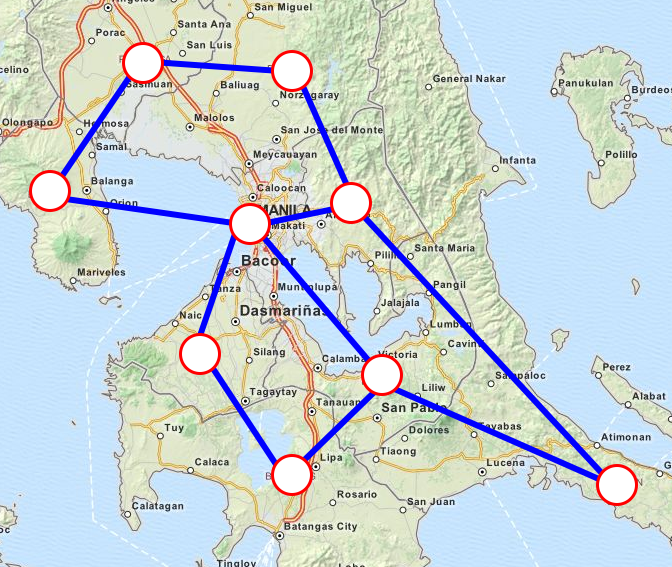
\includegraphics[height=75mm]{Images/intro2}\\
\end{center}
\end{frame}

\begin{frame}
\frametitle{Facility Location}
\begin{center}
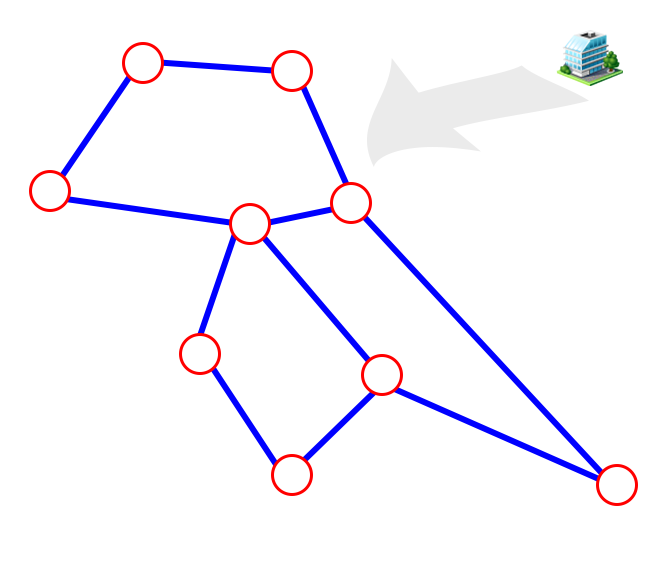
\includegraphics[height=75mm]{Images/intro3}\\
\end{center}
\end{frame}

\begin{frame}
\frametitle{Facility Location}
\begin{center}
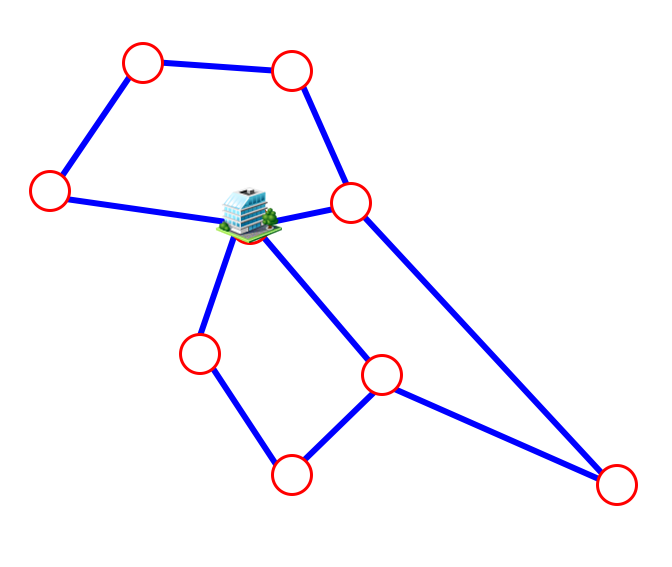
\includegraphics[height=75mm]{Images/intro4}\\
\end{center}
\end{frame}

\begin{frame}
\frametitle{Facility Location}
\begin{center}
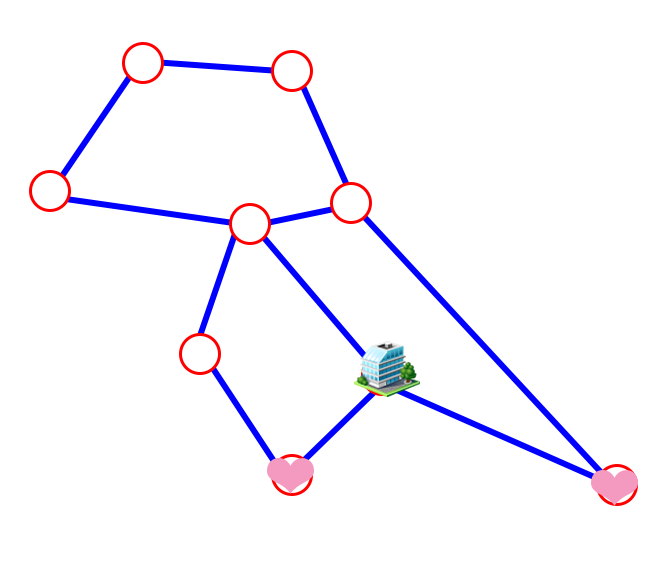
\includegraphics[height=75mm]{Images/intro5}\\
\end{center}
\end{frame}

\begin{frame}
\frametitle{Real World Applications}
\begin{itemize}
\item Placement of warehouses relative to production facilities and/or customers
\item Hospital/Fire station/ATM in a town
\item New classroom or building in a university
\item Placement of wireless hotspots in a building
\end{itemize}
\end{frame}

\section{Metric $p$-Center Problem}
\begin{frame}
\frametitle{Metric $p$-Center Problem}
\begin{itemize}
\item INSTANCE: A Complete Graph $G_c(V,E_c)$ and distances $d(v_i,v_j) \in \mathbb{N}$ satisfying 3 properties a metric space.
\item SOLUTION: A $p$-Center set, a subset $C \subseteq V$ and $\lvert C\rvert = p$
\item MEASURE: The maximum distance from a vertex to a nearest center 
$$
\max_{v \in V} \min_{c \in C} d(v,c)
$$
\end{itemize}
\end{frame}

\begin{frame}
\frametitle{Metric $p$-Center}
\begin{center}
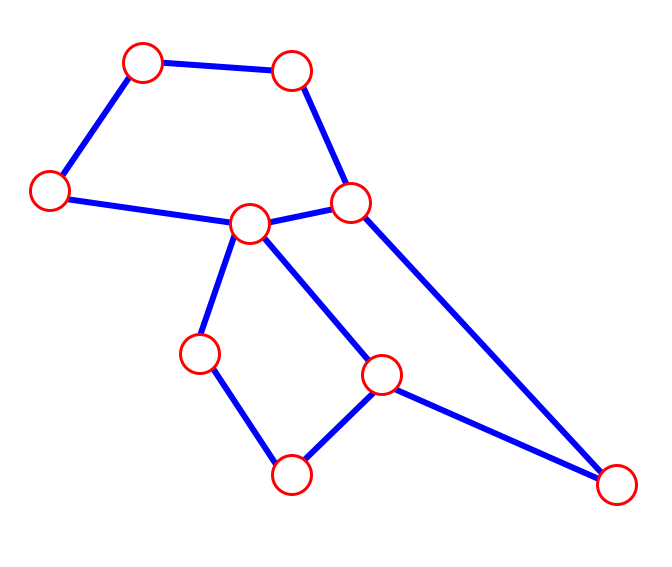
\includegraphics[height=75mm]{Images/metric1}\\
\end{center}
\end{frame}
\begin{frame}
\frametitle{Metric $p$-Center}
\begin{center}
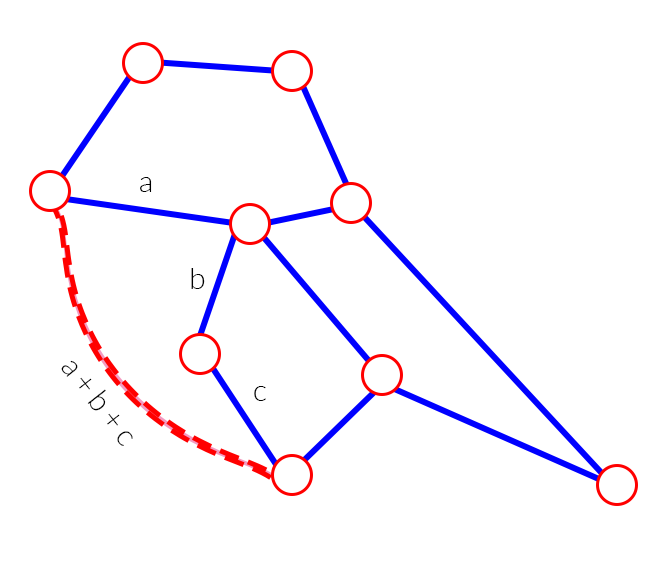
\includegraphics[height=75mm]{Images/metric2}\\
\end{center}
\end{frame}
\begin{frame}
\frametitle{Metric $p$-Center}
\begin{center}
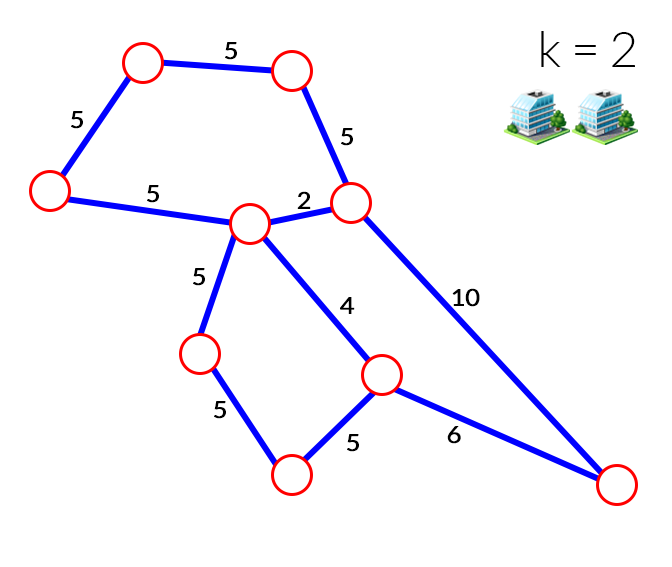
\includegraphics[height=75mm]{Images/metric3}\\
\end{center}
\end{frame}
\begin{frame}
\frametitle{Metric $p$-Center}
\begin{center}
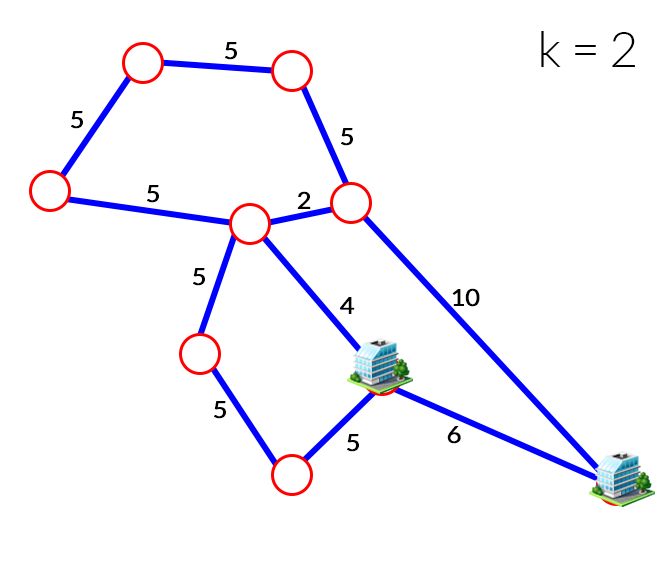
\includegraphics[height=75mm]{Images/metric4}\\
\end{center}
\end{frame}
\begin{frame}
\frametitle{Metric $p$-Center}
\begin{center}
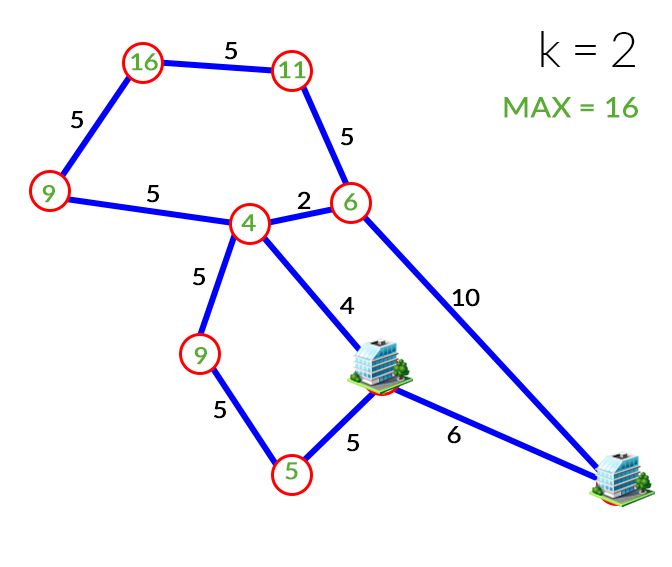
\includegraphics[height=75mm]{Images/metric5}\\
\end{center}
\end{frame}
\begin{frame}
\frametitle{Metric $p$-Center}
\begin{center}
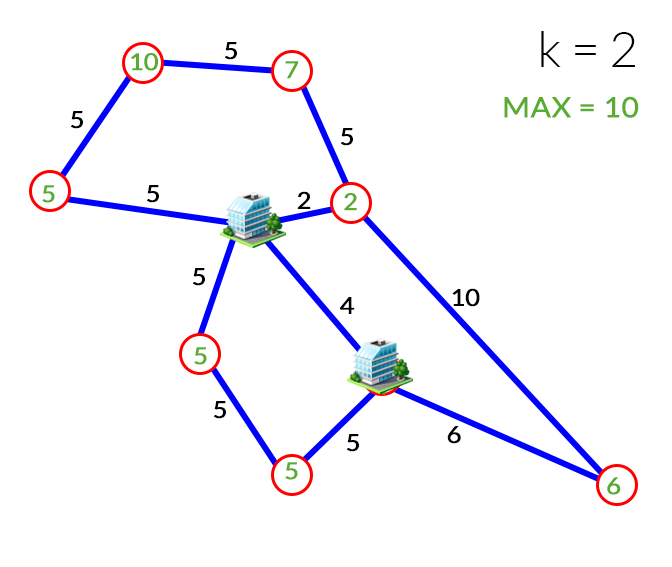
\includegraphics[height=75mm]{Images/metric6}\\
\end{center}
\end{frame}
\begin{frame}
\frametitle{Metric $p$-Center}
\begin{center}
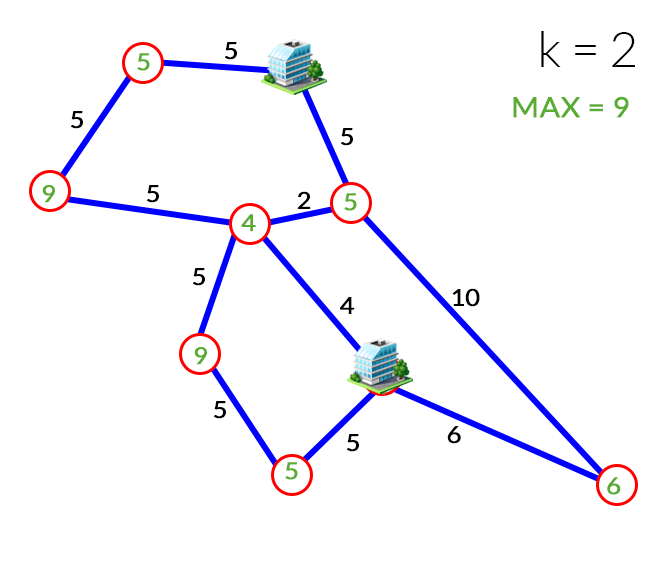
\includegraphics[height=75mm]{Images/metric7}\\
\end{center}
\end{frame}

\begin{frame}
\frametitle{Metric $p$-Center Problem}
\begin{center}
Metric $p$-Center Problem is \alert{NP-hard}.  
\end{center}
\end{frame}

\begin{frame}
\frametitle{Metric $p$-Center Problem}
\begin{center}
Finding an exact solution is \alert{difficult}  
\end{center}
\end{frame}

\begin{frame}
\frametitle{Metric $p$-Center Problem}
\begin{center}
Using heuristics to find a \alert{near-optimal} solutions is more practical.  
\end{center}
\end{frame}

\section{Ant Colony Optimization for $p$-center}
\begin{frame}
\frametitle{Ant Colony Optimization}
\begin{center}
Nature inspired algorithms based on the ability of \alert{ants} to find the \alert{optimal path} from home to food source.
\end{center}
\end{frame}

\begin{frame}
\frametitle{Ant Colony Optimization}
\begin{center}
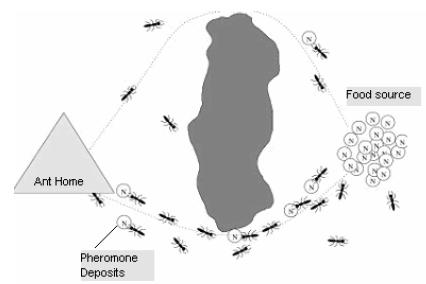
\includegraphics[height=60mm]{Images/ant1}\\
\tiny{\url{http://1.bp.blogspot.com/_jBmO8t-27_w/S9e2sUSS1VI/AAAAAAAACRc/yf8wyc81QvE/s1600/ant-vanet1.JPG}}
\end{center}
\end{frame}

\begin{frame}[fragile]
\frametitle{Ant Colony Optimization}
\begin{algorithm}[H]
\caption{Ant Colony Optimization}\label{alg:Ant Colony Optimization}
\begin{algorithmic}[1]

\State $Initialize Parameters$
\While{ $\neg Terminating Condition$}
\State $ConstructAntSolutions$
\State $UpdatePheromones$
\EndWhile
\end{algorithmic}
\end{algorithm}
\end{frame}

\begin{frame}
\frametitle{Parameters Initialization}
\begin{itemize}
\item Number of cities
\item Number of ants
\item Number of facilities
\item Max number of iterations
\end{itemize}
\end{frame}


\begin{frame}
\frametitle{Parameters Initialization}
\begin{itemize}
\item Each city initially has 0.01 pheromone level
\end{itemize}
\end{frame}

\begin{frame}
\frametitle{Parameters Initialization}
\begin{center}
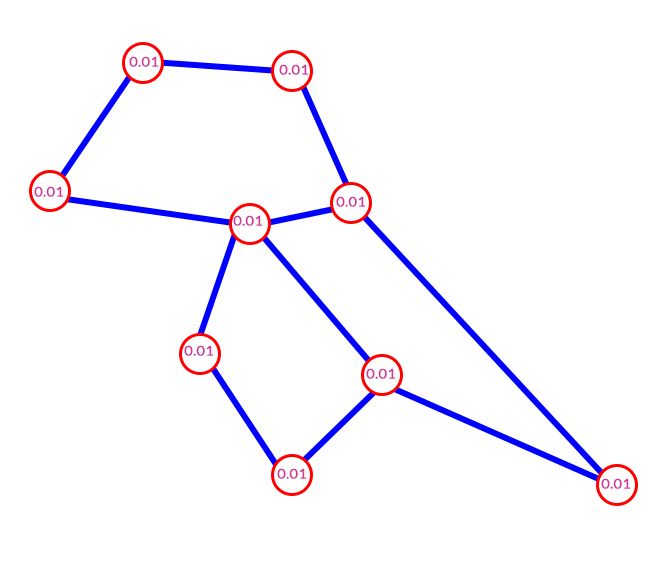
\includegraphics[height=75mm]{Images/pheromone1}\\
\end{center}
\end{frame}


\begin{frame}
\frametitle{Terminating Condition}
\begin{itemize}
\item Terminating condition is set as maximum number of iterations
\end{itemize}
\end{frame}

\begin{frame}
\frametitle{Ant Solution Construction}
\begin{itemize}
\item Each ant has its own \textit{solution storage}
\item An ant may only select a max number of facilities from all the cities
\item An ant \alert{probabistically} selects a city based on the current pheromone value in that location
\end{itemize}
\end{frame}

\begin{frame}
\frametitle{Ant City Selection}
\begin{itemize}
\item Probability of selecting city $x \in V$ from $G(V,E)$ as next city
$$
P(x) = \frac{\tau(x)^{\alpha} \times \eta(x)^{\beta}}{\sum_{v \in V} \tau(v)^{\alpha} \times \eta(v)^{\beta}}
$$
\item $\tau(x)$ is the pheromone level on city $x$
\item $\eta(x)$ is the attractiveness of selecting city $x$ \\(i.e. maximum distance of any city to city $x$)
\item $\alpha$ is the pheromone influence control parameter
\item $\beta$ is the attractiveness influence control parameter
\end{itemize}
\end{frame}

\begin{frame}
\frametitle{Ant City Selection}
\begin{center}
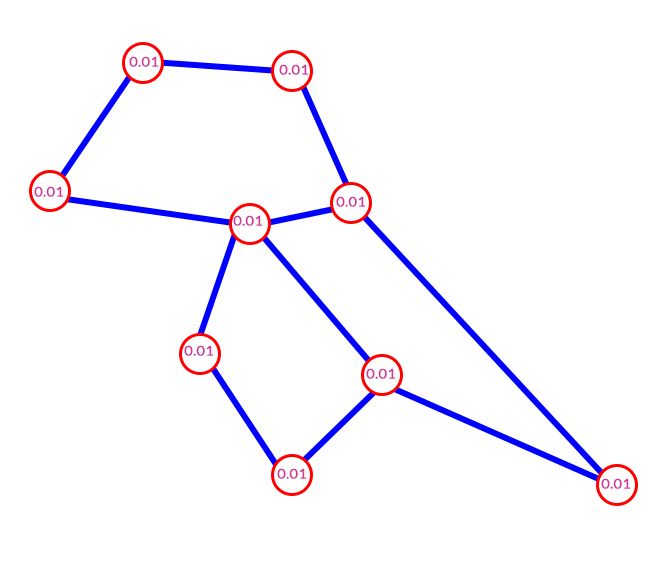
\includegraphics[height=75mm]{Images/pheromone1}\\
\end{center}
\end{frame}

\begin{frame}
\frametitle{Ant City Selection}
\begin{center}
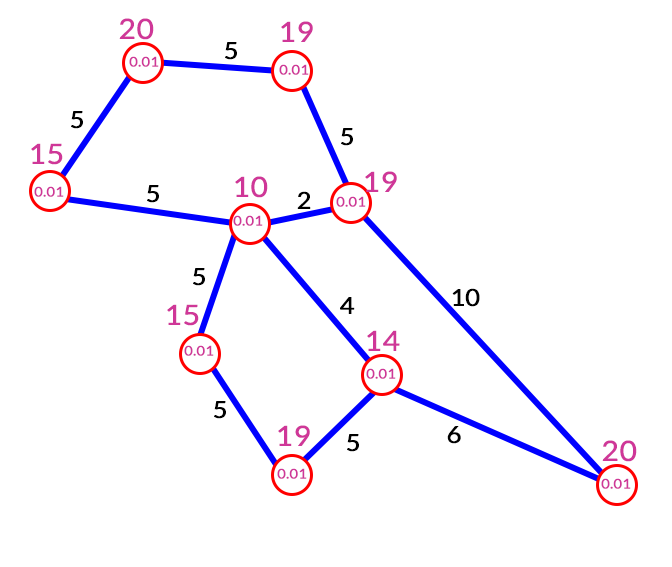
\includegraphics[height=75mm]{Images/pheromone2}\\
\end{center}
\end{frame}
\begin{frame}
\frametitle{Ant City Selection}
\begin{center}
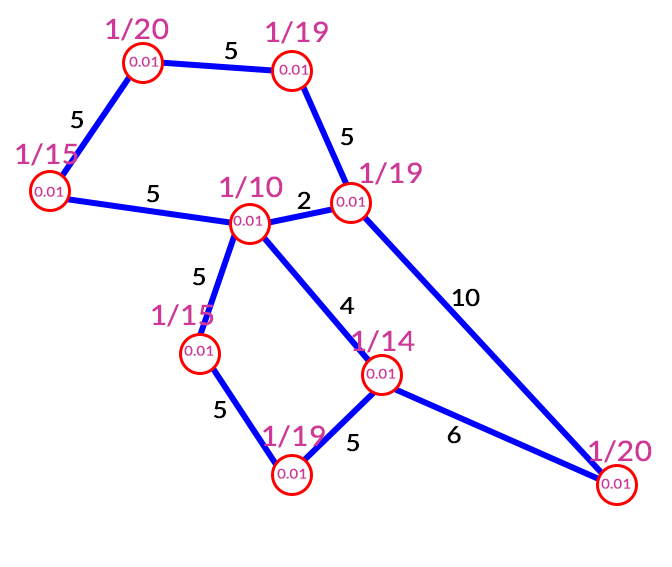
\includegraphics[height=75mm]{Images/pheromone3}\\
\end{center}
\end{frame}
\begin{frame}
\frametitle{Ant City Selection}
\begin{center}
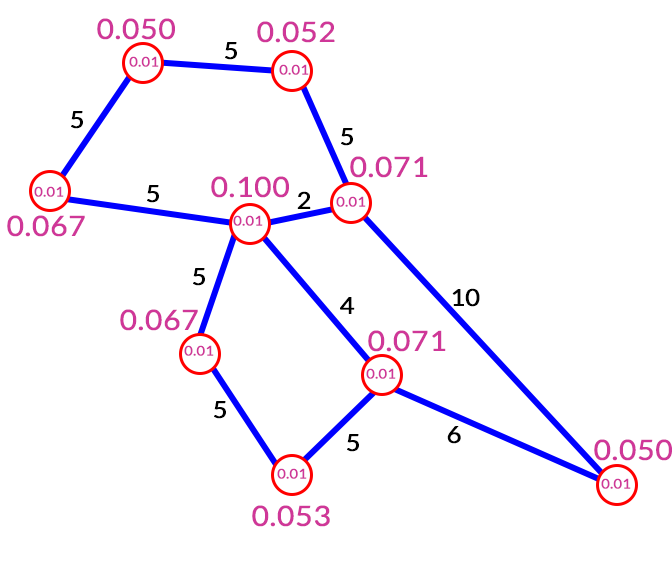
\includegraphics[height=75mm]{Images/pheromone4}\\
\end{center}
\end{frame}
\begin{frame}
\frametitle{Ant City Selection}
\begin{center}
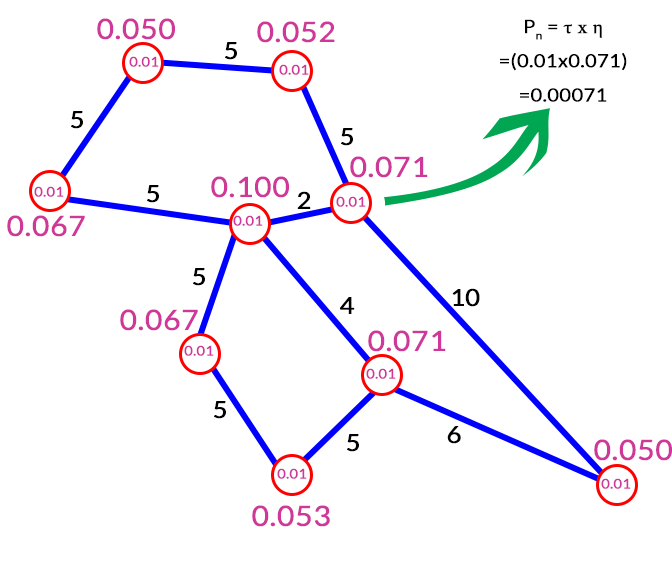
\includegraphics[height=75mm]{Images/pheromone5}\\
\end{center}
\end{frame}
\begin{frame}
\frametitle{Ant City Selection}
\begin{center}
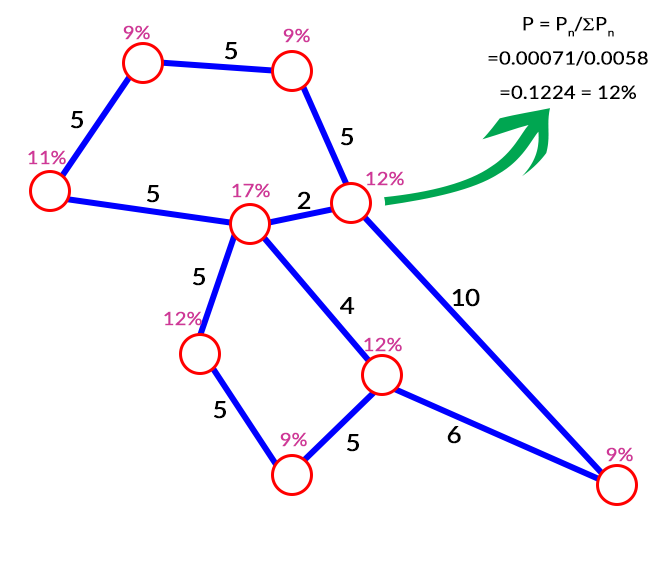
\includegraphics[height=75mm]{Images/pheromone6}\\
\end{center}
\end{frame}

\begin{frame}
\frametitle{Ant City Selection}
\begin{center}
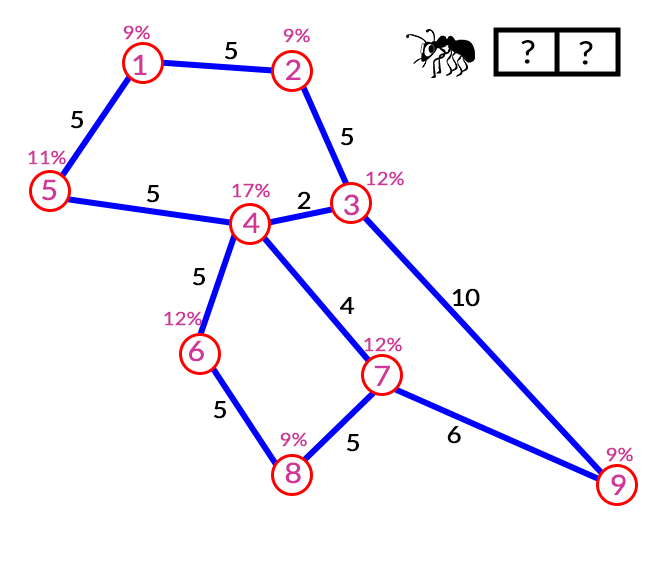
\includegraphics[height=75mm]{Images/antblack1}\\
\end{center}
\end{frame}
\begin{frame}
\frametitle{Ant City Selection}
\begin{center}
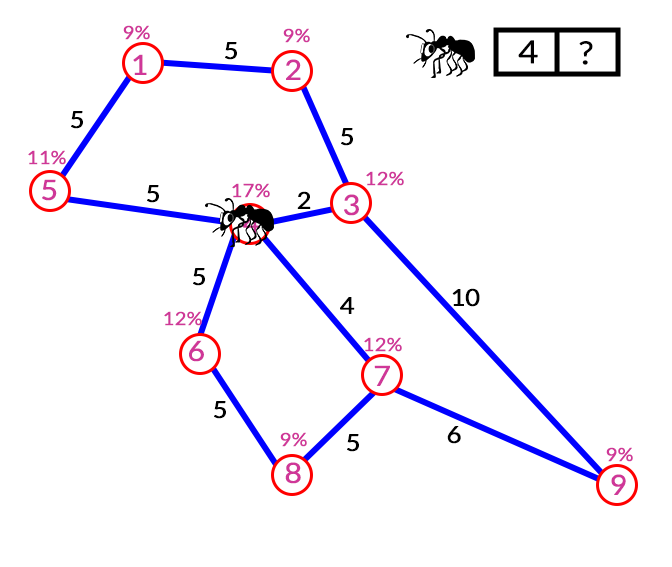
\includegraphics[height=75mm]{Images/antblack2}\\
\end{center}
\end{frame}
\begin{frame}
\frametitle{Ant City Selection}
\begin{center}
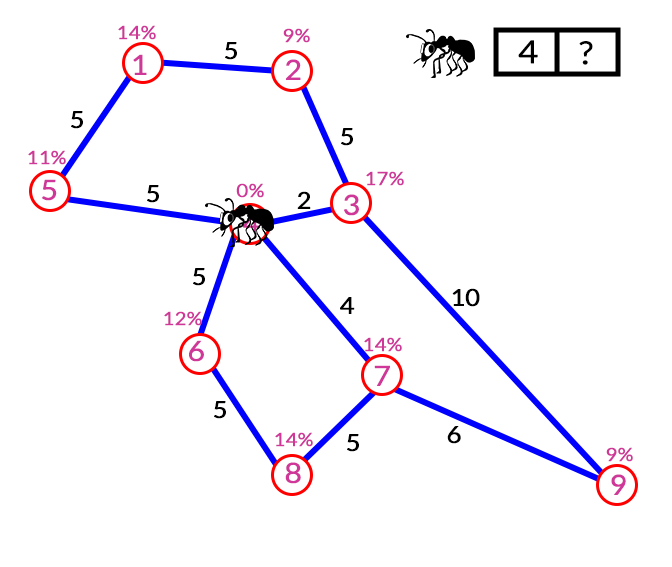
\includegraphics[height=75mm]{Images/antblack3}\\
\end{center}
\end{frame}
\begin{frame}
\frametitle{Ant City Selection}
\begin{center}
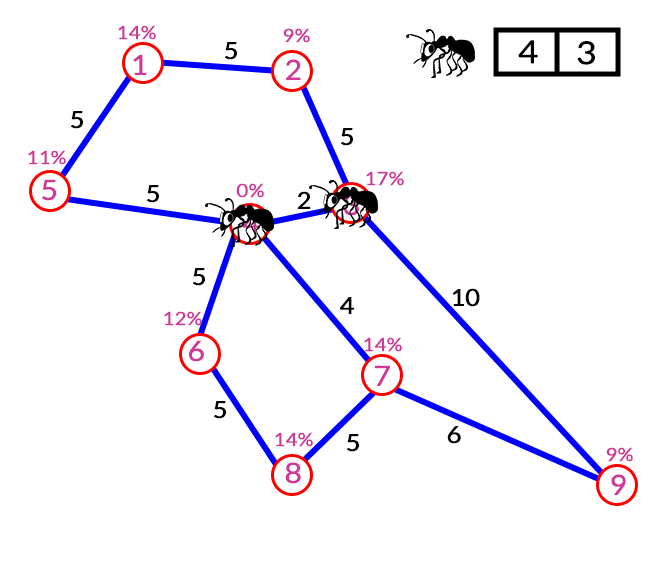
\includegraphics[height=75mm]{Images/antblack4}\\
\end{center}
\end{frame}

\begin{frame}
\frametitle{Ant City Selection}
\begin{center}
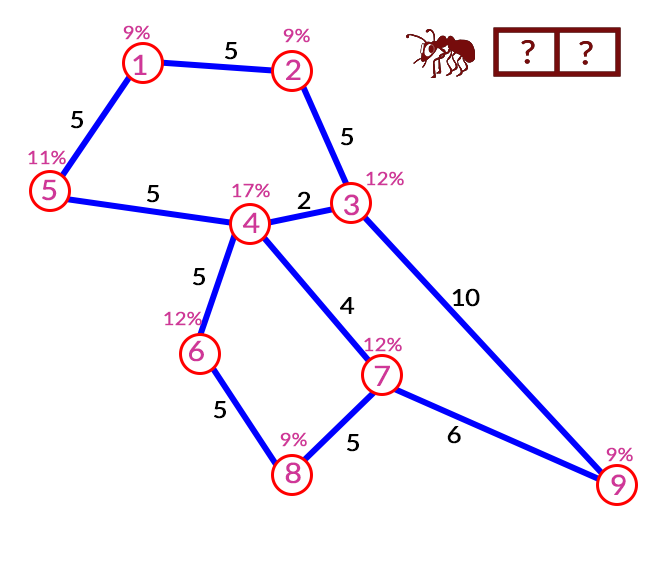
\includegraphics[height=75mm]{Images/antred1}\\
\end{center}
\end{frame}
\begin{frame}
\frametitle{Ant City Selection}
\begin{center}
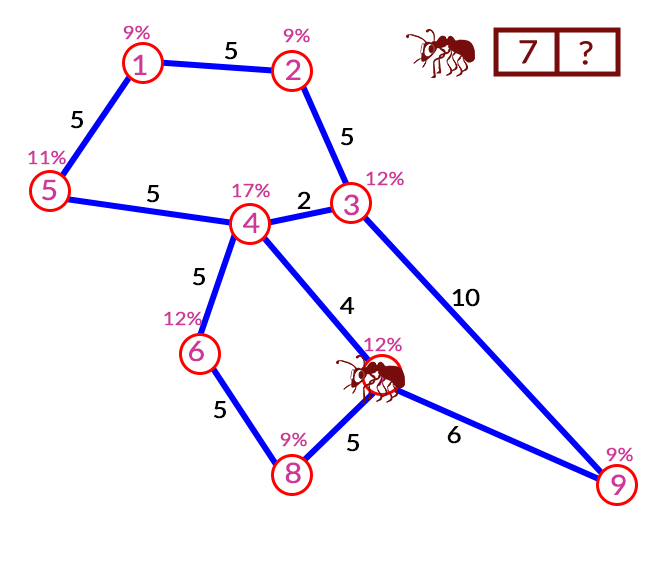
\includegraphics[height=75mm]{Images/antred2}\\
\end{center}
\end{frame}
\begin{frame}
\frametitle{Ant City Selection}
\begin{center}
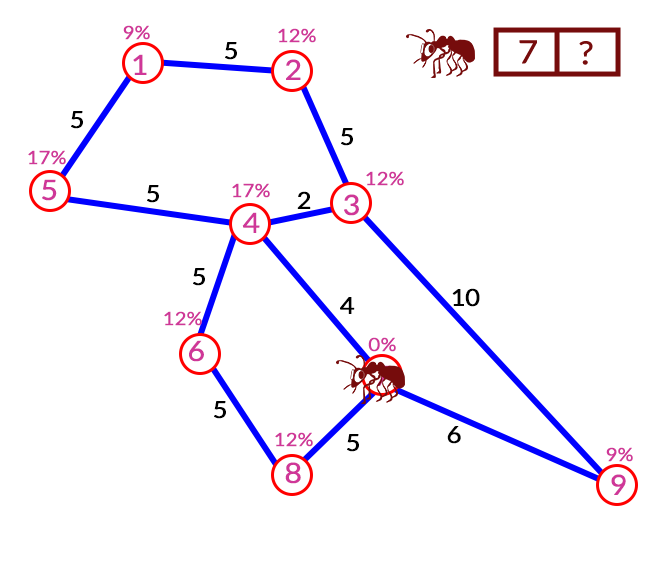
\includegraphics[height=75mm]{Images/antred3}\\
\end{center}
\end{frame}
\begin{frame}
\frametitle{Ant City Selection}
\begin{center}
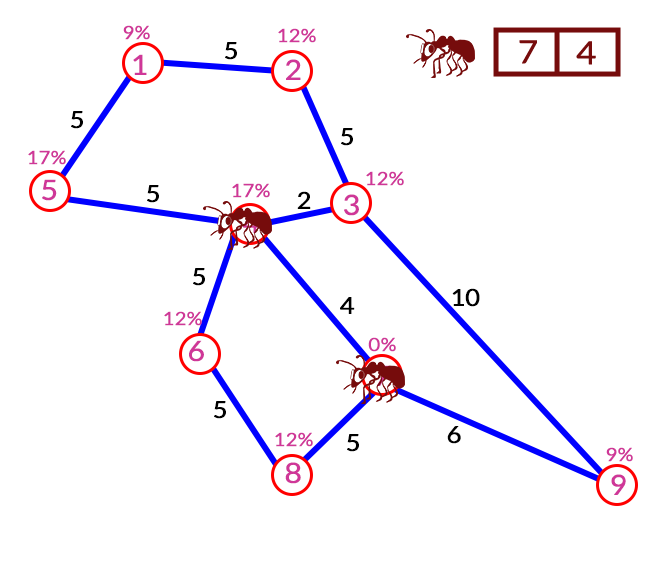
\includegraphics[height=75mm]{Images/antred4}\\
\end{center}
\end{frame}


\begin{frame}
\frametitle{Pheromone Update}
\begin{itemize}
\item Pheromones are updated when all ants have constructed their solutions
$$
\tau(x) \leftarrow (1 - \rho) \times \tau(x) + \sum\limits_{k \in K} \Delta\tau(k,x)
$$
\item $K$ is the set of ants
\item $(1-\rho)$ is the pheromone evaporation rate
\item $\Delta\tau(k,x)$ is the pheromone increase effect of ant $k$ to city $x$ 
$$\Delta\tau(k,x) = 
\begin{cases}
\dfrac{2}{\max_{v \in V}d(v,x)}	& \text{if } x \in C_{k}\\ 
0								& otherwise
\end{cases}
$$
\item $C_{k}$ is the solution of ant k where $C_{k} \subset V$
\end{itemize}
\end{frame}

\begin{frame}
\frametitle{Pheromone Update}
\begin{center}
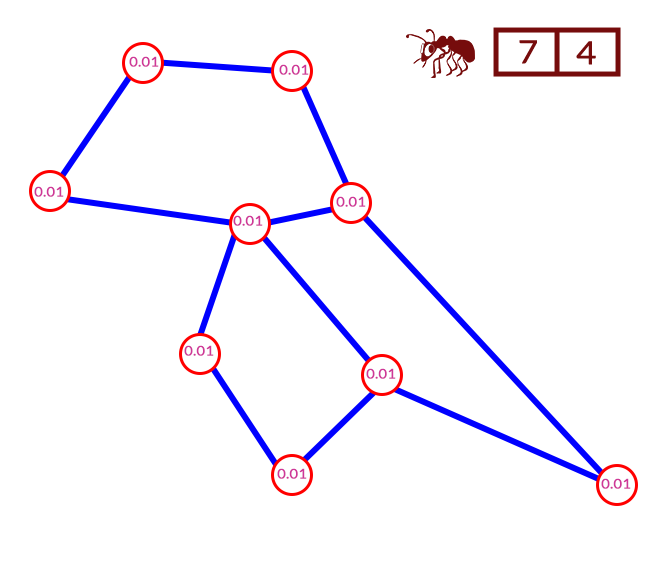
\includegraphics[height=75mm]{Images/increase1}\\
\end{center}
\end{frame}
\begin{frame}
\frametitle{Pheromone Update}
\begin{center}
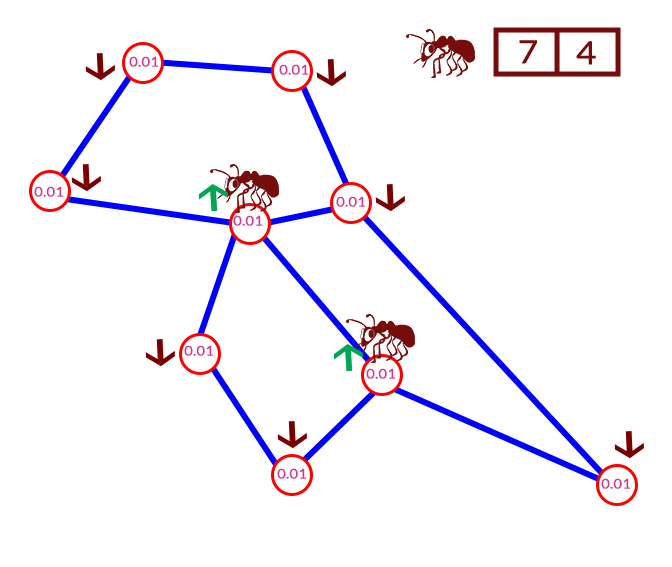
\includegraphics[height=75mm]{Images/increase2}\\
\end{center}
\end{frame}
\begin{frame}
\frametitle{Pheromone Update}
\begin{center}
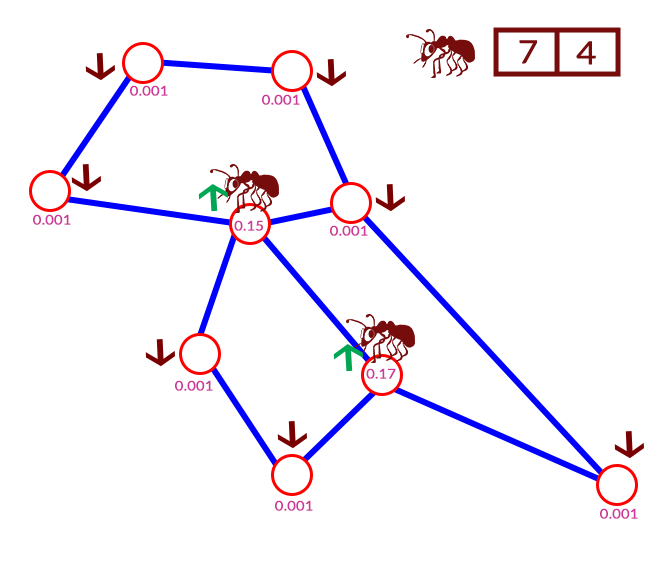
\includegraphics[height=75mm]{Images/increase3}\\
\end{center}
\end{frame}


\begin{frame}
\frametitle{Best Ant}
\begin{itemize}
\item Each ant remembers all of its selected cities based from previous steps
\item The ant that knows the best selection among its peers is considered the \alert{best ant} of the \alert{current iteration}
\item The best ant of the current iteration is compared with the \alert{global best ant}
\end{itemize}
\end{frame}

\begin{frame}
\frametitle{Ant Solution Quality}
\begin{itemize}
\item Based on the objective function of metric $p$-Center problem
$$\max_{v \in V}\{ \min_{c \in C} d(v,c)\}$$
\item The algorithm tries to \alert{minimize} that value by hoping that the ants will find the near-best solution
\end{itemize}
\end{frame}


\begin{frame}
\frametitle{Next Iteration}
\begin{itemize}
\item Repeat process above with the \alert{pheromone levels} from previous iteration
\item N generation ants affect N+1 generation ants by leaving the pheromones
\item Repeat until a stopping criterion is achieved
\end{itemize}
\end{frame}

\section{Experimentation}
\begin{frame}
\frametitle{Method}
\begin{center}
\begin{enumerate}
\item Input graph instances will be created.
\item Complete Graph will be induced from corresponding input graph instances.
\item Exact IP or LP-Relaxed solution on metric $p$-Center for the input instance will be solved.
\item Approximate solutions are found using variants of Ant Colony Algorithms for metric $p$-Center.
\end{enumerate}
\end{center}
\end{frame}

\begin{frame}
\frametitle{Input Graph Instances}
\begin{center}

		Random graph generation using a created program.
		
\end{center}
\end{frame}


\begin{frame}
\frametitle{Complete Graph Induction from Input Test Cases}
\begin{itemize}
\item Input test will be parsed and represented as an adjacency matrix/list.
\item Edge completion will be done using all pairs shortest path algorithms
\begin{itemize}
	\item Floyd-Warshall all pairs shortest path OR
	\item Dijkstra's Algorithm on all vertices
\end{itemize}

\end{itemize}
\end{frame}

\begin{frame}
\frametitle{Integer Programming Formulation: Decision Variables}
\begin{itemize}
\item Let $z$ be the maximum distance from a city/vertex to a city/vertex with an open facility
\item Let
	$
	y_j = 
	\begin{cases}
	1	& \text{if a facility is opened at city } j \\
	0	& \text{otherwise }
	\end{cases}
	$
\item Let $x_{ij}= 
	\begin{cases}
	1	& \text{if city } i  \text{ is assigned at facility in city } j \\
	0	& \text{otherwise }
	\end{cases}
	$ 
\end{itemize}
\end{frame}

\begin{frame}
\frametitle{Integer Programming Formulation}
$$
Minimize\texttt{ }z
\label{eq:$p$-Center Problem IP Objective Function}
$$

Subject to:
$$
\begin{aligned}
\sum_j^n y_{j} = p & \texttt{     } & \texttt{        }
\end{aligned}
\label{eq:$p$-Center Problem IP Facility Count Constraint}
$$

$$
\begin{aligned}
\sum_j^n x_{ij} = 1 & \texttt{     } & \forall i
\end{aligned}
\label{eq:$p$-Center Problem IP City-Facility Assignment Constraint}
$$

$$
\begin{aligned}
x_{ij} \leq y_j & \texttt{     } & \forall i,j
\end{aligned}
\label{eq:$p$-Center Problem IP Open Facility Constraint}
$$

$$
\begin{aligned}
z \geq \sum_j^n d_{ij}x_{ij} & \texttt{     } & \forall i
\end{aligned}
\label{eq:$p$-Center Problem IP Largest Possible Z-value}
$$

$$
\begin{aligned}
x_{ij},y_j \in \{0,1\} & \texttt{     } & \forall i,j
\end{aligned}
\label{eq:$p$-Center Problem IP Integer 0-1 Constraint}
$$

\end{frame}

\begin{frame}
\frametitle{Integer Programming Formulation: Constraints}
$$
\begin{aligned}
\sum_j^n y_{j} = p & \texttt{     } & \texttt{        }
\end{aligned}
\label{eq:$p$-Center Problem IP Facility Count Constraint}
$$
\begin{center}
This ensures that exactly $p$ facilities are opened.
\end{center}
\end{frame}

\begin{frame}
\frametitle{Integer Programming Formulation: Constraints}
$$
\begin{aligned}
\sum_j^n x_{ij} = 1 & \texttt{     } & \forall i
\end{aligned}
\label{eq:$p$-Center Problem IP City-Facility Assignment Constraint}
$$
\begin{center}
This ensures that that city $i$ must only be serviced by a single facility.
\end{center}
\end{frame}

\begin{frame}
\frametitle{Integer Programming Formulation: Constraints}
$$
\begin{aligned}
x_{ij} \leq y_j & \texttt{     } & \forall i,j
\end{aligned}
\label{eq:$p$-Center Problem IP Open Facility Constraint}
$$
\begin{center}
This ensures that city $i$ cannot be assigned/serviced by a city $j$ with no open facility.
\end{center}
\end{frame}

\begin{frame}
\frametitle{Integer Programming Formulation: Constraints}
$$
\begin{aligned}
z \geq \sum_j^n d_{ij}x_{ij} & \texttt{     } & \forall i
\end{aligned}
\label{eq:$p$-Center Problem IP Largest Possible Z-value}
$$
\begin{center}
This ensures that the value of $z$ is the maximum distance from any city that needs to be serviced by an open facility.
\\[3ex]
We want to \alert{minimize} this value.
\end{center}
\end{frame}


%\begin{frame}
%\frametitle{Bibliography}
%\bibliographystyle{abbrv}
%\bibliography{refs}
%\end{frame}

\end{document}
